\documentclass[11pt, a4paper]{article}
\usepackage[utf8]{inputenc}
\usepackage[T1]{fontenc}
\usepackage{framed}
\usepackage[french]{babel}
\usepackage{tabularx}
\usepackage[T1]{fontenc}
\usepackage{lmodern}
\usepackage{graphicx}
\usepackage{fancyhdr}
\usepackage{amsfonts}
\usepackage{verbatim}
\usepackage{listings}
\usepackage{float}

\usepackage{xcolor}
\usepackage{listings}


\newcommand\defeq{\mathrel{\stackrel{\makebox[0pt]{\mbox{\normalfont\tiny def}}}{=}}}

\pagestyle{fancy}
\renewcommand\headrulewidth{0pt}
\fancyhead[L]{\emph{Groupe Amuat - Maalel - Poleya}}
\fancyhead[R]{Projet Logiciel Transversal}
\fancyfoot[L]{\emph{Rapport de Jalon 1}}
\fancyfoot[R]{\today}

\begin{document}

\lstset{literate=
{é}{{\'e}}1
{à}{{\`a}}1
{â}{{\^a}}1
}
\definecolor{orange}{rgb}{0.8,0.4,0.0}
\definecolor{darkblue}{rgb}{0.0,0.0,0.6}
\definecolor{cyan}{rgb}{0.0,0.6,0.6}
\lstdefinelanguage{JSON}
{
   basicstyle=\normalsize,
   columns=fullflexible,
   showstringspaces=false,
   commentstyle=\color{gray}\upshape,
   morestring=[b]",
   morestring=[s]{>}{<},
   morecomment=[s]{<?}{?>},
   stringstyle=\color{orange},
   identifierstyle=\color{darkblue},
   keywordstyle=\color{blue},
   morekeywords={string,number,array,object}% list your attributes here
}

\title{Rapport de jalon de Projet Logiciel Transversal}

\maketitle

\tableofcontents
\newpage
 
\section{Objectif}

\subsection{Présentation générale}

L’objectif de ce projet est la réalisation d’un jeu de plateforme inspiré de “Dofus”, avec des règles et des designs simplifiés

\subsection{À propos du jeu}

\subsubsection{Règles du jeu}

Ce jeu possède deux modes: un mode exploration et un mode combat. Le joueur se déplace librement sur la carte en mode exploration et peut passer un mode combat en décidant d’affronter un ennemi présent sur cette même carte en cliquant dessus. La finalité de ce jeu d’aventure est de combattre des ennemis afin de gagner en expérience et de là augmenter de niveau.

\subsubsection{Description générale}

Voici la description générale du jeu à réaliser :

\begin{enumerate}
\item Deux modes : 
	\begin{enumerate}
		\item Mode exploration
		\item Mode combat
	\end{enumerate}
\item Des acteurs jouables et non jouables
	\begin{enumerate}
		\item Deux personnages (féminin, masculin)
		\item Cinq créatures (ennemis)
	\end{enumerate}
\item Six plateformes
	\begin{enumerate}
		\item Trois cartes pour le mode exploration
		\item Trois cartes pour le mode combat (générées à partir des cartes d'exploration)
	\end{enumerate}
\item Trois menus
	\begin{enumerate}
		\item Démarrer (Nouvelle partie, création de Personnage ...)
		\item Pause (Quitter, sauvegarder ...)
		\item Infos Personnage
	\end{enumerate}
\end{enumerate}

\subsubsection{Description détaillée}
Modes : 
\begin{itemize}
\item Exploration: Dans ce mode le joueur peut se déplacer librement sur la carte en cliquant sur une case, lancer un combat en se dirigeant vers une créature présente sur la carte.
\item Combat: Dans ce mode il s’agit d’un duel entre le joueur et une adversaire (créature/monstre). Ce mode prend fin lorsqu’un des acteurs  meurt.\\*
\end{itemize}


Voici la description détaillée du jeu à réaliser :

\begin{figure}[h]
  \centering
  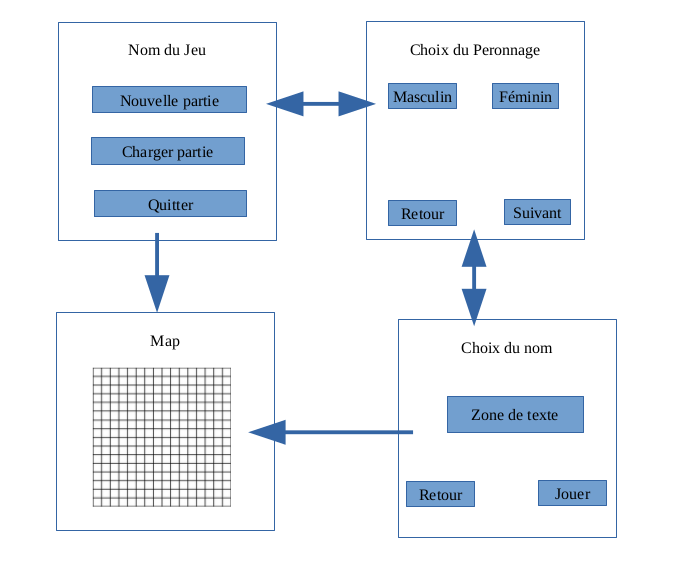
\includegraphics[scale=0.5]{img/MenuDemarrer.png}
  \caption{\emph{Organisation et maquettes des menus}}
\end{figure}

Au lancement du jeu, le menu démarrer s’affiche et trois options sont disponibles. Le bouton “Nouvelle partie” permet de lancer une nouvelle partie et redirige l’utilisateur vers un menu nommé “Choix du personnage. Le bouton “Charger partie” permet de lancer une partie enregistrée auparavant et redirige l’utilisateur vers la carte du jeu. Le bouton “Quitter” permet de mettre fin à l’exécution du jeu.
Dans le menu “Choix du personnage”, deux choix s’offrent à l’utilisateur soit un personnage masculin ou soit un personnage féminin. Une fois cette sélection effectuée l’utilisateur est dirigé vers un menu nommé “Choix du nom” permettant d’attribuer un pseudo au personnage retenu. Enfin, le bouton “Jouer” présent dans ce menu permet d’accéder à la plate-forme de jeu.

Menu Pause : 

\begin{figure}[h]
  \centering
  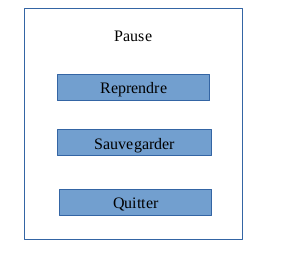
\includegraphics[scale=1]{img/MenuPause.png}
  \caption{\emph{Menu de pause}}
\end{figure}

Au cours du jeu (hormis en mode de combat) via le bouton ‘échap’ du clavier, l’utilisateur peut accéder au menu “Pause” qui propose à ce dernier trois options: reprendre la partie du jeu en cours, sauvegarder la partie de jeu en cours et quitter le jeu en cours. \\*

Menu Infos personnage : 

\begin{figure}[H]
  \centering
  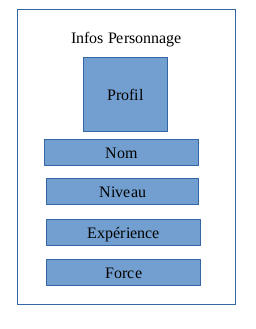
\includegraphics[scale=1]{img/MenuInfosPerso.png}
  \caption{\emph{Menu Infos}}
\end{figure}

Au cours du jeu (hormis en mode de combat) via le bouton ‘tab’ du clavier, l’utilisateur peut accéder au menu “Infos Personnage” qui contient tous les informations (nom, niveau, expérience, force, profil) sur le personnage du joueur.\\*

Cartes :

Deux types de cartes sont présents dans ce jeu : trois cartes dédiées au mode exploration et trois cartes dédiées au mode combat.

\begin{figure}[H]
  \centering
  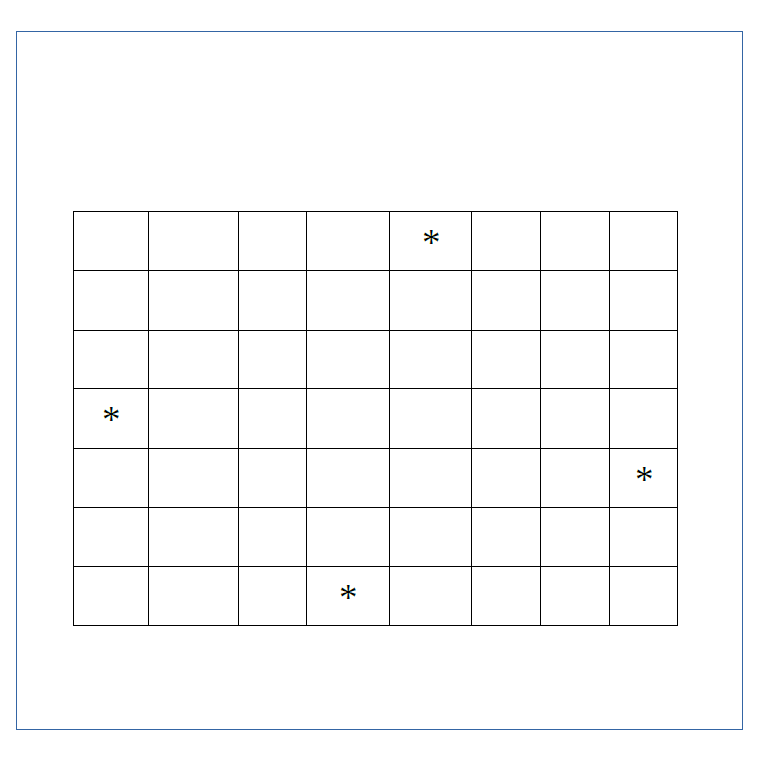
\includegraphics[scale=0.7]{img/CarteExplo.png}
  \caption{\emph{Modèle de carte en navigation}}
\end{figure}

\begin{itemize}
\item Le changement de carte s’effectue via les points d’accès (*)
\item Sur la carte exploration, il y a présence du personnage (joueur) et des ennemis (créatures)\\
\end{itemize}

Carte de combat :

\begin{figure}[H]
  \centering
  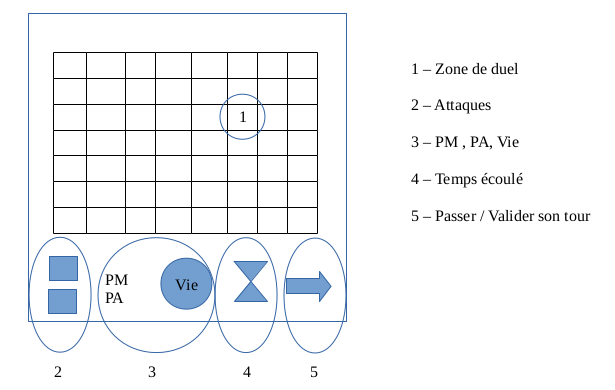
\includegraphics[scale=0.5]{img/CarteCombat.png}
  \caption{\emph{Modèle de carte en combat}}
\end{figure}

Sur la carte combat, il y a deux principales zones :

\begin{itemize}
\item Une zone de combat : 
	\begin{itemize}
	\item Dimension de la zone de duel : 12 carreaux * 10 carreaux
	\item Effets visuels: Assombrissement du fond et zoom sur la zone de combat
	\item Effets sonores: changement de musique
	\end{itemize}
\item une zone commandes/actions :
	\begin{itemize}
	\item une attaque corps à corps
	\item une attaque à distance
	\item Points de Mouvement (nombre de cases pouvant être parcourues par tour), Points d’Action (nombre d’attaques pouvant être lancées par tour) et Points de Vie dépendent du niveau du joueur
	\item Temps de jeu par tour de 60 secondes
	\item Touche “Passer/Valider” permet de mettre fin à son tour
	\end{itemize}
\end{itemize}

Les différents acteurs présents dans ce jeu sont :
	
\begin{itemize}
\item Deux personnages: un masculin et un féminin
\item Cinq créatures (I.A)
\end{itemize}

Le joueur augmente de niveau en faisant des duels et en gagnant de l’expérience et les créatures ont des niveaux différents allant de 1 à 10.\\*

Evolution du personnage :\\*

\begin{tabular}{|c|c|c|c|c|c|}
\hline
	Niveau & Vie & PM & PA & Exp \\
\hline
   1 & 100 & 3 & 6 & 100 \\
\hline
   2 & 150 & 4 & 7 & 200 \\
\hline
   3 & 200 & 5 & 8 & 300 \\
\hline
   4 & 250 & 6 & 9 & 400 \\
\hline
   5 & 300 & 7 & 10 & 500 \\
\hline
   6 & 350 & 8 & 11 & 600 \\
\hline
   7 & 400 & 9 & 12 & 700 \\
\hline
   8 & 450 & 10 & 13 & 800 \\
\hline
   9 & 500 & 11 & 14 & 900 \\
\hline
   10 & 550 & 12 & 15 & 1000 \\
 \hline 
\end{tabular}\\ \\*

Ce tableau résume l’évolution des paramètres Vie, PM, PA et Exp en fonction du niveau du personnage.\\*

\section{Description et conception des états}

\subsection{Description des états}

Notre jeu consiste principalement au déplacement d’un personnage sur une carte et à l’affrontement de monstres sur cette même carte. Le jeu évolue d’un état à un autre et cela de manière continue en fonction des actions du joueur. Ces différents états sont décrits de manière globale dans les paragraphes suivants.

\subsubsection{Etat Général}

Un état de jeu est formée par un ensemble d’éléments mobiles (heros, monstres) et d’un ensemble d’éléments fixes (cases “vide”, cases “acces”). Tout élément est défini par :
\begin{itemize}
\item Sa position (coordonnées x et y)
\item Son identifiant TypeID qui permet de distinguer la nature (la classe) de l’élément
\end{itemize} 

\subsubsection{Etat éléments mobiles}
Héros jouables et monstres sont définis dans deux classes héritant de trois classes chacune, pour définir leurs caractéristiques dans un système flexible mais néanmoins résilient au changement. Tout d’abord la classe “\textbf{Élément}” définit la position actuelle, selon x et y, de l’élément concernée. Cette classe permet également l’inclusion dans les listes définies par la classe “\textbf{ListeElements}”, qui servira à l’enregistrement de tous les éléments de jeu. Ensuite la classe “\textbf{Mobile}” permet de définir la direction actuelle de déplacement de l’élément, essentielle pour la gestion des sprites par le package de rendu. Enfin la classe “\textbf{Personnage}” comporte les principales caractéristiques des être vivants du jeu : Niveau, Vie, Force, Points d’action, Points de Mouvement, Attaque à distance et Attaque au corps à corps. Ces dernières sont définies par une autre classe “\textbf{Attaque}” qui peut être instanciée pour définir les dégâts infligés par une attaque ou le coût en point d’action de l’attaque. À part ces éléments communs, on notera que la gestion de l’expérience a motivé la distinction entre les classes “\textbf{Heros}” et “\textbf{Monstre}”

\subsubsection{Etat éléments fixes}

Les déplacements sur une carte s’effectuent de case en case d’une grille, et le changement de carte s’effectue sur des points d’accès disséminés de part et d’autre de la carte. Ces notions sont retranscrites dans l’existence d’une classe “\textbf{Grille}” contenant des éléments soit “vide” soit des points d’accès vers une carte suivante. Cette grille est composée d’une liste d’éléments et est représentée par la classe “\textbf{Grille}” qui hérite de “\textbf{ListeElements}”, mais qui ne sera composée que de “\textbf{Statique}”, classe héritant de “\textbf{Element}”. La séparation en deux classes “\textbf{Vide}” et “\textbf{Acces}” permet de rajouter un attribut vers lequel l’élément non statique pointe.

\subsubsection{Etat mode de jeu}

	Un élément important du gameplay résidant dans la distinction entre le mode “combat” et le mode “exploration”, la classe “Combat” définit les principaux états propres au mode “combat” : l’existence d’un ordre de tour de jeu entre les différents personnages et d’un timer limitant la durée d’un tour. En outre, un attribut “EnCombat” contenue par la classe “\textbf{Etat}” indique si les joueurs se trouvent actuellement en combat ou en exploration. \\*\\

\begin{tabularx}{\textwidth}{ |c|X| }
\hline
	\textbf{Classe} & \textbf{Rôle} \\
\hline

   Etat & Cette classe permet de définir un état de jeu.

Attribut(s): personnages, grille, combat, enCombat, visiteur, mapActuel\newline
Méthode(s): Etat(), ~Etat(), getStatutGrille(), getPersonnage(), getRefPersonnage(), loadGrille(), getGrille(), getEnCombat(), setEnComabt(), rajouterPerso(), enleverPerso(), getRefCombat(), getMapActuel(), setMapActuel(), getPerso(), getPersoSize(), getGrilleSize(),getTile()
 \\
\hline

   ListeElements & Cette classe permet de définir un objet de type “ListeElements”. Cette liste permet d’enregistrer tous les éléments mobiles et statiques nécessaires à l’état du jeu.

Attribut(s): elements,factory
\newline
Méthode(s): ListeElements(), ~ListeElements(), size(), getElement(), setElement(), isPerso(), ajoutElement()
 \\
\hline

   GrilleElements & Cette classe permet de définir une liste d’élements de type “GrilleElements”. Elle hérite de la classe “ListeElements”. Cette classe permet de construire une map de taille donnée (longueur * largeur) et d’y accéder aux cases sous forme matricielle. Pour faciliter le traitement, les cases sont enregistrées sous forme de liste d’éléments.

Attribut(s): longueur, largeur
\newline
Méthode(s): GrilleElements(), getLongueur(), getLargeur(), isAcces(), setCase(), charger(),setLongueur(), setLargeur(), ajoutCaseAcces()
 \\
\hline

   Combat & Cette classe permet de définir un objet de type “Combat”. Elle gère la gestion d’un combat (fonctionnement tour par tour).

Attribut(s): timerDebutTour, listeTour, tourActuel
\newline
Méthode(s): combat(), ~Combat(), createListe(), tourSuivant(), getTimerDebutTour()
 \\
\hline

   ElementFactory & Cette classe permet de définir un objet de type “ElementFactory” comme défini dans les standards de Design Pattern.

Attribut(s): timerDebutTour, listeTour, tourActuel
\newline
Méthode(s): combat(), ~Combat(), createListe(), tourSuivant(), getTimerDebutTour()
 \\
\hline

   IElementAlloc & Cette classe abstraite permet de définir un objet de type “IElementAlloc”.
\newline
Méthode(s): \textbf{IElementAlloc()}, \textbf{newInstance()}
 \\*
\hline

\end{tabularx} 

\begin{tabularx}{\textwidth}{ |l|X| }
\hline
   HerosAlloc & Cette classe permet de définir un objet de type “HerosAlloc”. Elle hérite de la classe “IElementAlloc”.

Attribut(s): id
\newline
Méthode(s): ElementAlloc(), newInstance()
 \\
\hline

   MonstreAlloc & Cette classe permet de définir un objet de type “MonstreAlloc”. Elle hérite de la classe “IElementAlloc”.

Attribut(s): id
\newline
Méthode(s): ElementAlloc(), newInstance()
 \\
\hline

   VideAlloc & Cette classe permet de définir un objet de type “VideAlloc”. Elle hérite de la classe “IElementAlloc”.

Attribut(s): id
\newline
Méthode(s): ElementAlloc(), newInstance()
 \\
\hline

   AccesAlloc & Cette classe permet de définir un objet de type “AccesAlloc”. Elle hérite de la classe “IElementAlloc”.

Attribut(s): id
\newline
Méthode(s): ElementAlloc(), newInstance()
 \\
\hline

   IVisiteur & Cette classe abstraite permet de définir un objet de type “Ivisiteur” selon le modèle du Pattern Visiteur qui permet d’accéder à des informations via des pointeurs.

Attribut(s): pHeros, pVide, pAcces, pMonstre, lastType
\newline
Méthode(s): visiter()
 \\
\hline

   Visiteur & Cette classe permet de définir un objet de type “Visiteur”. Elle hérite de la classe “Ivisiteur”.
\newline
Méthode(s): Visiter(), getpHeros(), getpMonstre(), getpAcces(), getpVide()
 \\
\hline

   IAccepteVisite & Cette classe abstraite permet de définir une interface du type “IaccepteVisite”.
\newline
Méthode(s): accepte()
 \\
\hline

   Element & Cette classe permet de définir un objet de type “Element”. Cet élément est caractérisé par une position sur la grille de coordonnées (x;y) et d’un type d’identifiant selon le type énuméré « TypeID » qui permet d’identifier le type d’élément selon l’ID défini. Cette classe est inclue dans la classe « ListeElements »

Attribut(s): x, y, typeID, elemID
\newline
Méthode(s): Element(), ~Element(), \textbf{getTypeID()}, \textbf{accepte()}, getX(), getY(), setX(), setY(), getElemID(), setElemID()
 \\
\hline

\end{tabularx}\\ \\*

\begin{tabularx}{\textwidth}{ |l|X| }
\hline
   Statique & Cette classe abstraite permet de définir un élément de type “Statique”. Elle est la classe mère des classes « Acces » et « vide » qui sont les deux éléments statiques du jeu.
\newline
Méthode(s): Statique(), \textbf{isAcces()}, \textbf{accepte()}, \textbf{getTypeID()}, isStatic(), getTile()
 \\
\hline

   Mobile & Cette classe abstraite permet de définir un élément de type “Mobile”. Elle est la classe mère de « Personnage » qui représente les éléments mobiles du jeu.

Attribut(s): joueur, direction, timer, enDeplacement
\newline
Méthode(s): Mobile(), \textbf{isJoueur()}, \textbf{accepte()}, \textbf{getTypeID()}, isStatic(), getDirection(), setDirection(), getEnDeplacement(), setEnDeplacement, getTimer(), setTimer()
 \\
\hline

   Personnage & Cette classe abstraite permet de définir un élément mobile de type “Personnage”. Elle hérite de la classe “Mobile”.

Attribut(s): typePersonnage, force, niveau, ptAction, ptMouvement, vie, attaqueDistance, attaqueCAC, etatPerso
\newline
Méthode(s): Personnage(), ~Personnage(), \textbf{isJoueur()},\textbf{ accepte()}, \textbf{getTypeID()}, getTypePersonnage(), getForce(), getNiveau(), getPA(), getPM(), getVie(), getAttaqueDistance(), getAttaqueCAC(), getEtatPerso(), setTypePersonnage(), setForce(), setNiveau(), setPA(),setPM(), setVie(), setAttaqueDistance(), setAttaqueCAC(), setEtatPerso()
 \\
\hline

   Attaque & Cette classe permet de définir un objet de type “Attaque”.

Attribut(s): typeAttaque, degat, coutPA
\newline
Méthode(s): Attaque(), ~Attaque(), getCoutPA(), setCoutPA()
 \\
\hline

   Vide & Cette classe permet de définir un élément fixe de type “Vide”. Elle hérite de la classe “Statique”.
\newline
Méthode(s): Vide(), isAcces(), getTypeID(), accepte()
 \\
\hline

   Acces & Cette classe permet de définir un élément fixe de type “Acces”. Elle hérite de la classe “Statique”.
\newline
Méthode(s): Acces(), isAcces(), getTypeID(), accepte()
 \\
\hline

   Heros & Cette classe permet de définir un élément mobile de type “Heros”. Elle hérite de la classe “Personnage”.
   
Attribut(s): experience
\newline
Méthode(s): Heros(), isJoueur(), getExp(), setExp(), accepte()
 \\
\hline

   Monstre & Cette classe permet de définir un élément mobile de type “Monstre”. Elle hérite de la classe “Personnage” tous ses attributs.
\newline
Méthode(s): Monstre(), isJoueur(), getTypeID(), accepte()
 \\
\hline

\end{tabularx}\\ \\*

\subsubsection{Diagramme des classes d'état}

Légende des couleurs:

\begin{itemize}

\item Vert: Correspond à l’ensemble des classes Etat et ListeElements ainsi que sa classe fille
\item Rouge: Correspond à la classe Combat
\item Marron: Correspond à l’ensemble des classes ElementFactory et IElementAlloc ainsi que ses classes filles selon un Pattern design Factory
\item Orange: Correspond à la classe Element et ses classes fille Statique, Mobile et Personnage
\item Violet: Correspond à la classe Attaque
\item Bleu: Correspond à l’ensemble des classes définies selon le modèle du Pattern design Visiteur
\item Jaune: Correspond aux dernières classes fille de la classe Element (Heros, Monstre, Vide et Acces)
\item Blanc: Correspond à l’ensemble des classes de type Énumération

\end{itemize}

\begin{figure}[H]
  \centering
  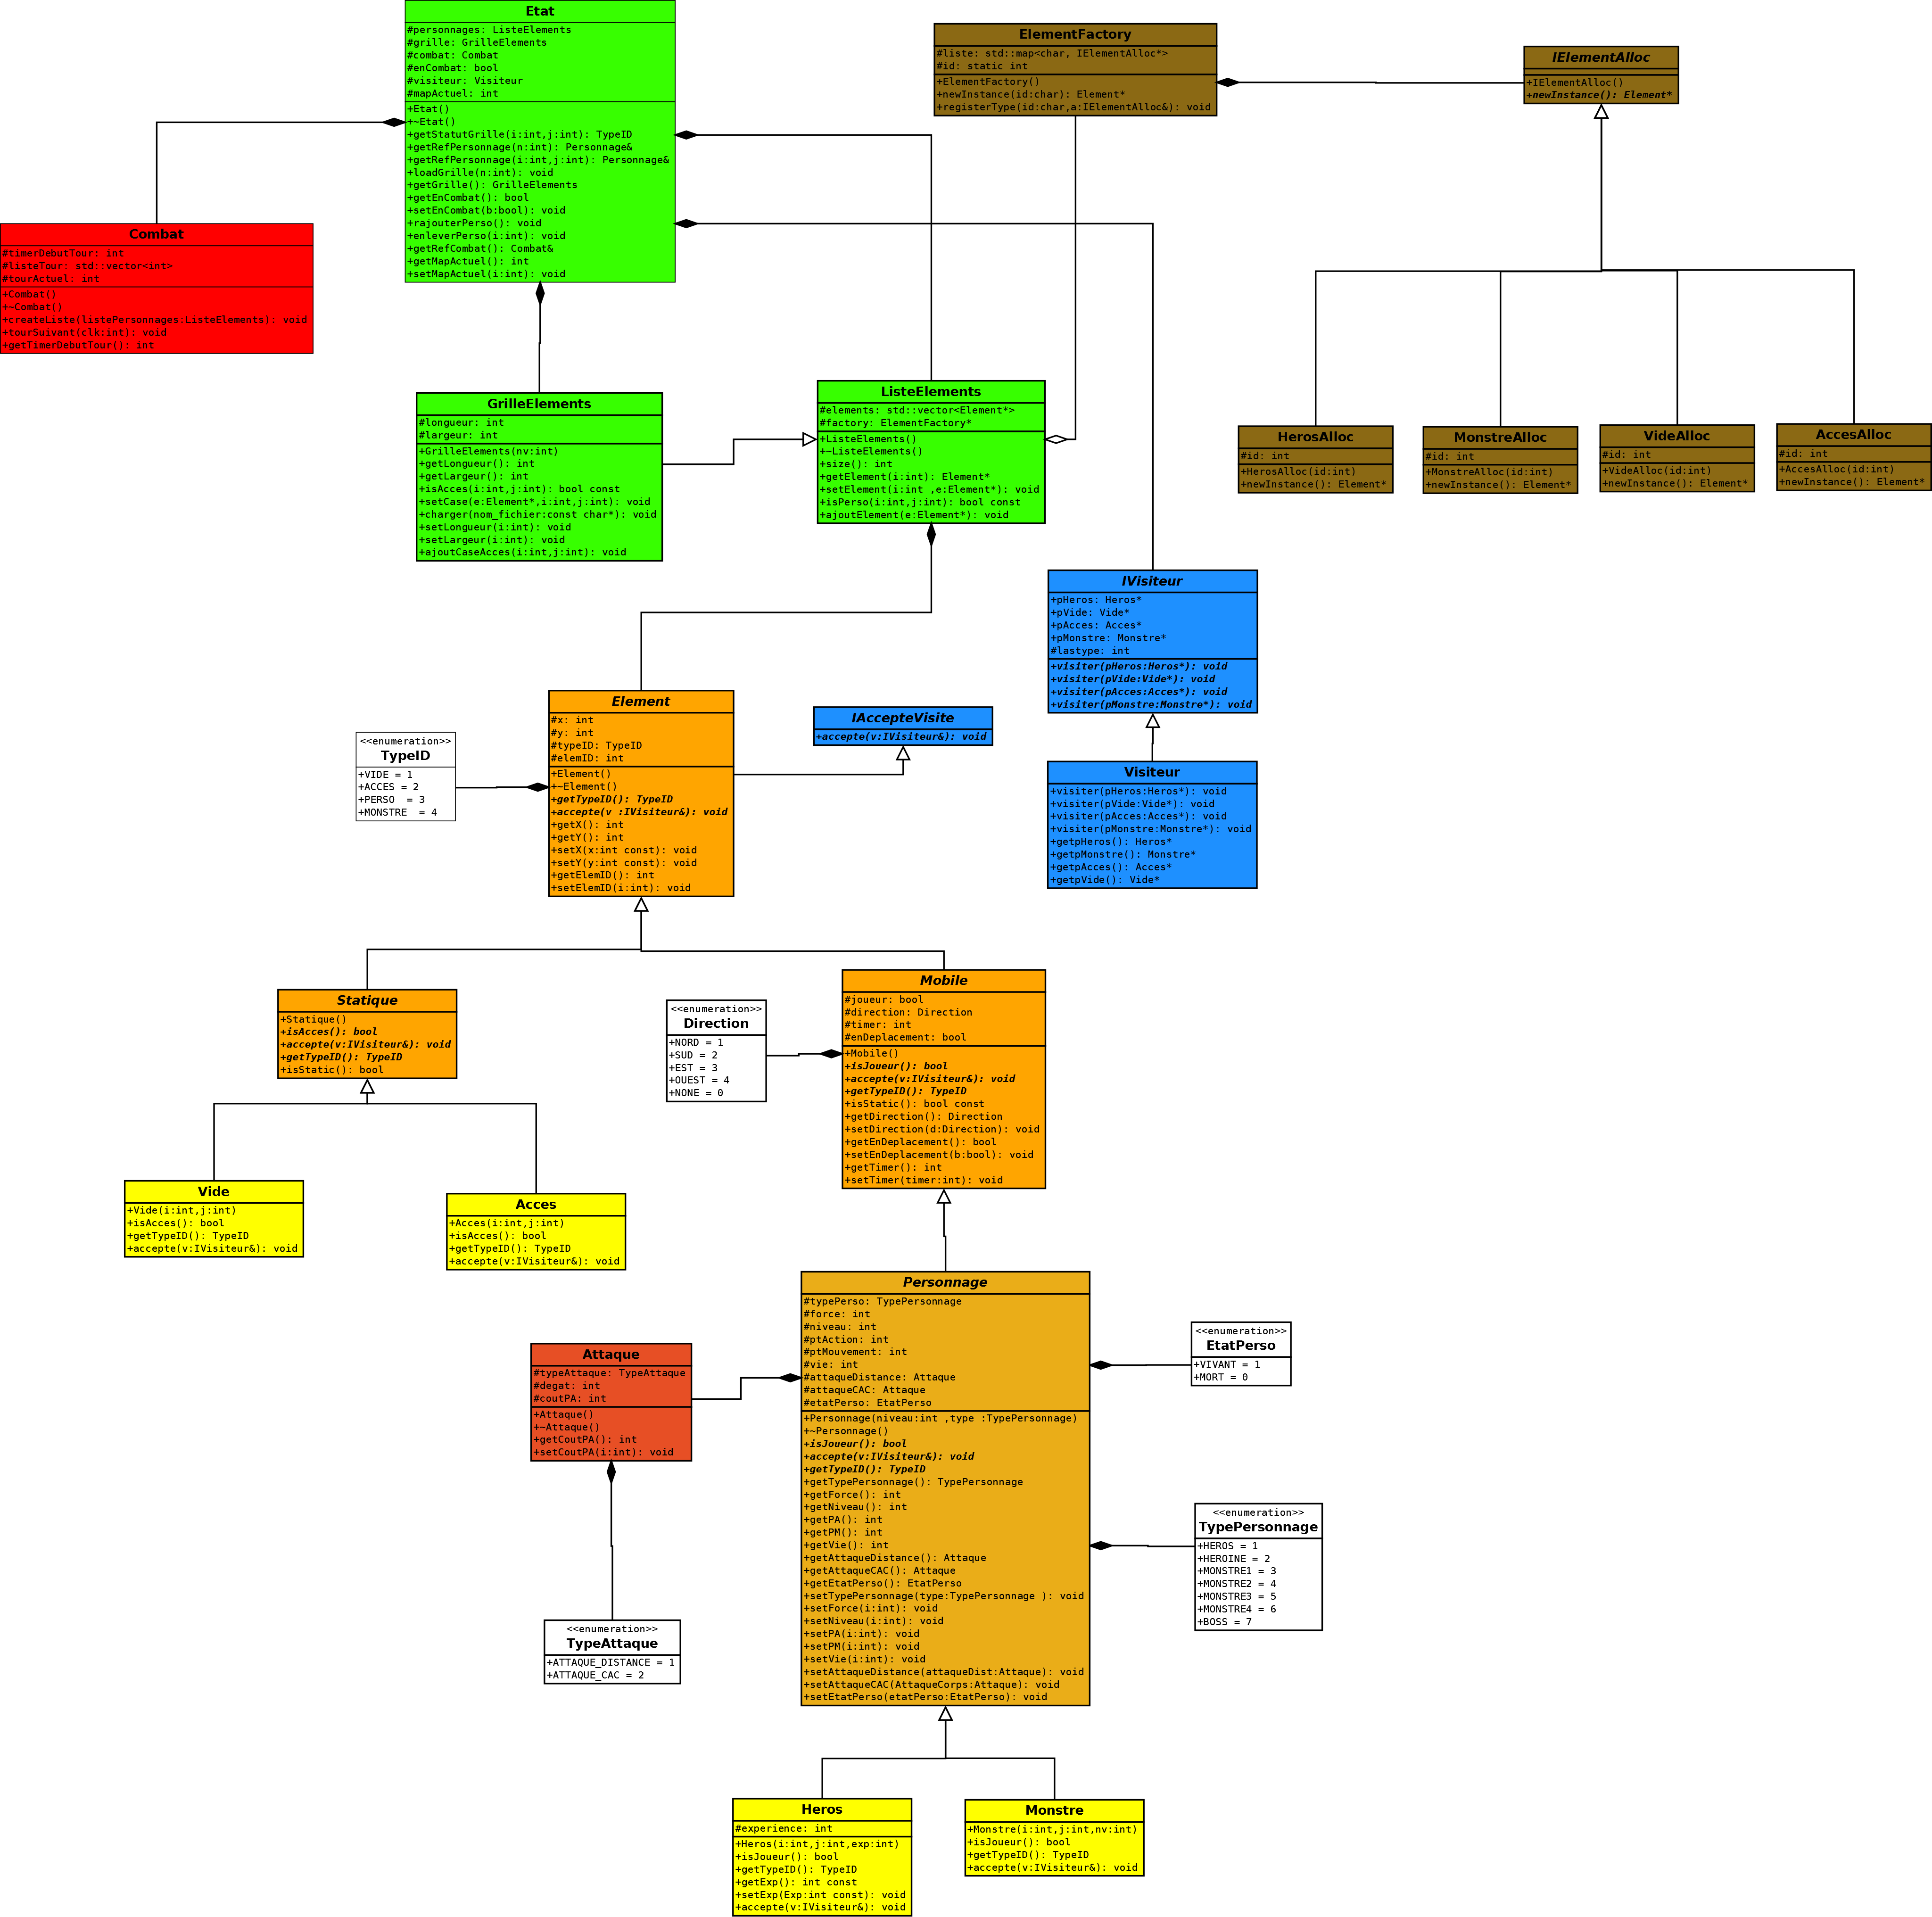
\includegraphics[scale=0.05]{img/state.png}
  \caption{\emph{Diagramme de classe du package etat du projet}}
\end{figure}

\section{Rendu}

\subsection{Stratégie de rendu d'un état}

Une stratégie relativement simple est choisie pour réaliser le rendu d’un état du jeu. Cette stratégie consiste à segmenter le rendu en deux plans: un plan pour la carte (contenant tous les éléments statiques) et un second plan pour les éléments mobiles (personnages).

	Une structure basée selon un Pattern Observer est utilisé afin de faire le lien entre le package State et le package Render. En effet, l’objectif de cette structure est d’observer l’état du jeu à rendre et d’apporter les changements survenus. Pour ce faire, l'implantation de six classes sont nécessaires:

Classes Observable et Observer:  ces classes appartiennent au Pattern Observer et ont pour but d'observer les changements survenus sur l'état du jeu et de les notifier au rendu. Ces classes font le lien entre le package Etat et le package Rendu.

Classe Rendu: cette classe centralise les différents plan du rendu. Elle permet de mettre à jour le rendu d'un état de jeu. Elle est associée à différentes classes qui sont: RenduGrille, RenduPerso.

Classe Parseur: cette classe permet d’accéder aux différentes textures utilisées pour le rendu du jeu en passant par une lecture de fichiers .txt. Le chargement de ces textures se fait à l’aide de tableaux d’entiers qui sont ensuite exploités dans les classes du package Render.

\subsection{Conception logiciel}

Le taleau ci dessous permet de résumer l’ensemble des classes utiles et présentes pour définir un rendu d'un état de jeu ainsi que leur rôle respectif.

\begin{tabularx}{\textwidth}{ |l|X| }
\hline
   \textbf{Nom} & \textbf{Role}
 \\
\hline

   Observable & Cette classe permet d'observer l'état du jeu.

Attribut(s): observers
\newline
Méthode(s): notifyObservers(), registerObserver()
 \\
\hline

   Observer & Cette classe permet de mettre à jour le rendu en fonction des changements survenus dans l'état du jeu.
   
Méthode(s): run()
 \\
\hline

   Rendu & Cette classe permet de gérer l'ensemble des plan du rendu à mettre à jour.

Attribut(s): rg, rp
\newline
Méthode(s): run(), Rendu()
 \\
\hline

   RenduGrille & Cette classe permet de gérer le rendu de la carte du jeu (background).

Attribut(s): level, vertices, tileset
\newline
Méthode(s): dessin(), charger(), RenduGrille(), ~RenduGrille()
 \\
\hline

   RenduPerso & Cette classe permet de gérer le rendu des personnages.

Attribut(s): vertices, tileset
\newline
Méthode(s): dessin(), RenduPerso(), ~RenduPerso()
 \\
\hline

   Parseur & Cette classe permet d’accéder à la lecture d’un fichier .txt qui spécifie les textures pour les personnages et les cartes du jeu.
\newline
Méthode(s): parsingMap(), parsingTextures(), trim(), ftos(), parsingString()
 \\
\hline

\end{tabularx}\\ \\*

Diagramme de classe :

\begin{figure}[H]
  \centering
  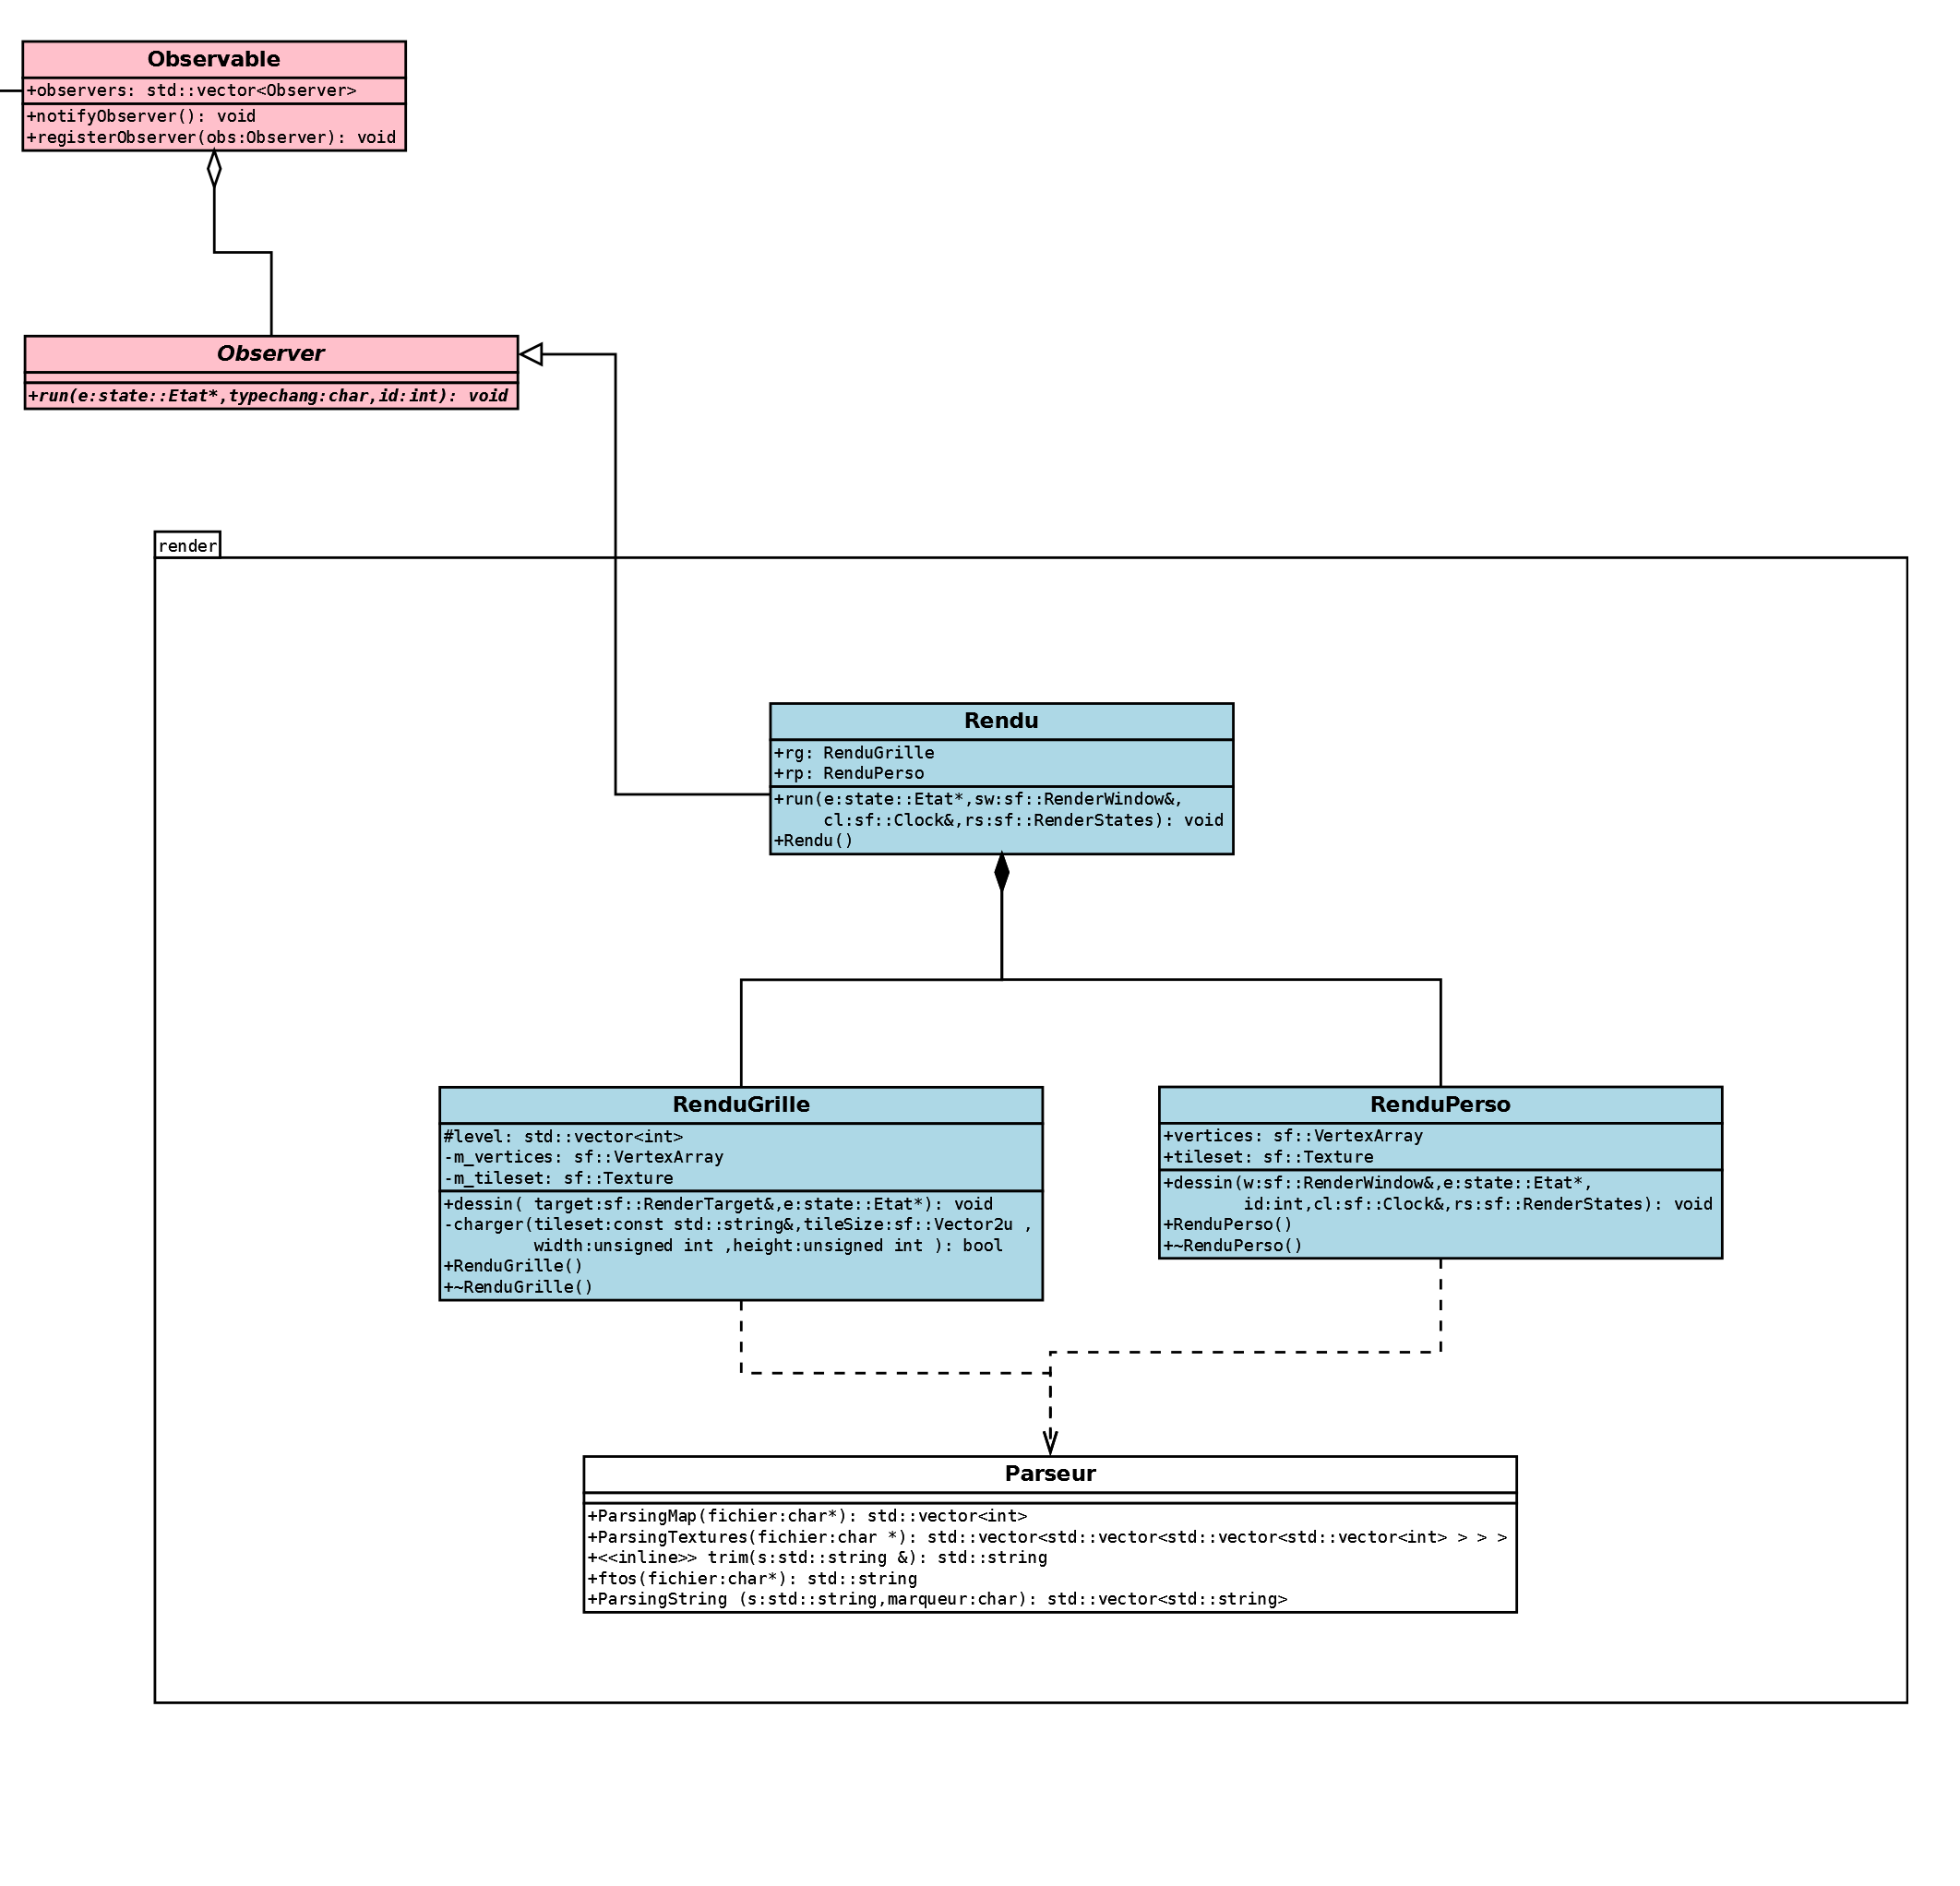
\includegraphics[scale=0.13]{img/render.png}
  \caption{\emph{Package render}}
\end{figure}

\subsection{Exemple de rendu}

\begin{figure}[H]
  \centering
  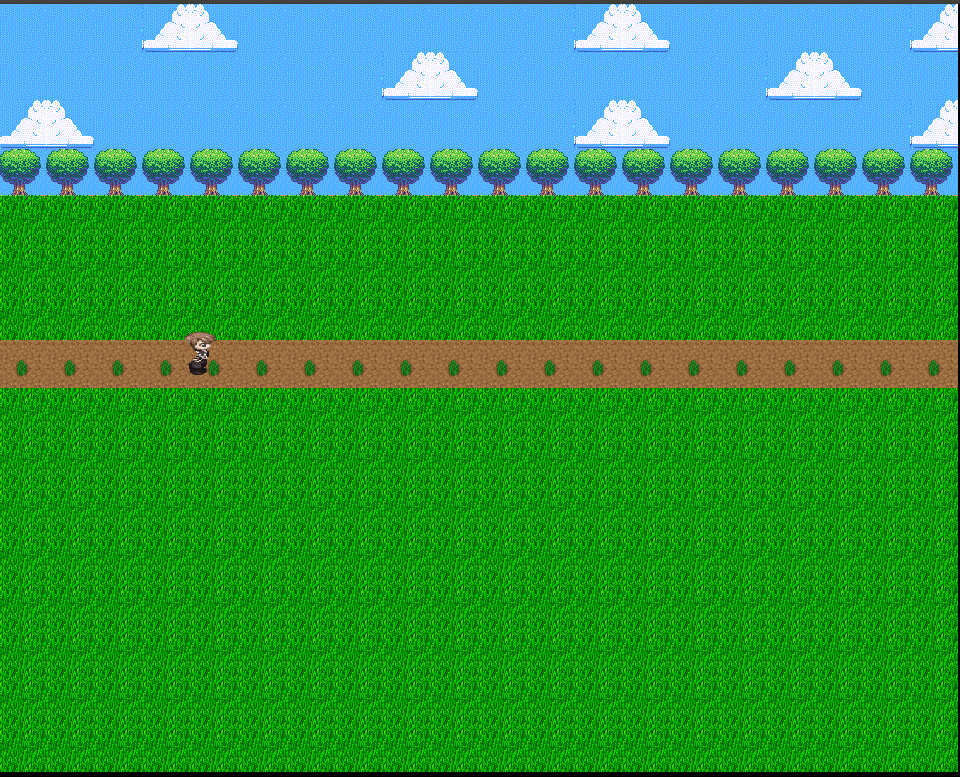
\includegraphics[scale=0.4]{img/rendu.png}
  \caption{\emph{Exemple de rendu}}
\end{figure}


\newpage
\section{Règles de changement d'états et moteur de jeu}
\subsection{Horloge principale}

Les changements d'états s'effectuent suivant une horloge principale. Ainsi, le jeu passe directement d'un état à un autre sans passer par un état intermédiaire. Cette horloge principale est lancée dès le début du jeu dans la fonction main. À chaque création de commandes une lecture du temps (sf::Time) est effectuée sur l'horloge principale. De plus, les déplacemements des personnages sont calibrés suivant l'horloge principale.

\subsection{Changements d'états extérieurs}

Les changements extérieurs provoqués par des commandes extérieures comme par exemple l'utilisation de la souris. En effet, à chaque intervention extérieures (souris, clavier) une commande associée à l'action désirée est créée. Cette commande est ensuite ajoutée à une liste de commandes qui sera exécutée par la suite par le moteur de jeu selon les règles du jeu.

\subsection{Changements d'états autonomes}

Les changements d'états autonomes sont réalisés à chaque mise à jour d'un état. Ces changements d'états autonomes sont principalement présents en mode Combat, en effet voici les actions effectuées de manière autonome:
\begin{enumerate}
 \item À chaque début de tour de jeu, tous les paramètres du joueur est mise à jour (Vie, PM, PA).
 \item À chaque déplacement du joueur, les points de mouvement sont modifiés en conséquence.
 \item À chaque utilisation d'attaque du joueur, les points d'action sont modifiés en conséquence.
 \item À chaque dégat subit par une attaque, les points de vie du joueur sont modifiés en conséquence.
 \item Une fois que le temps imparti pour un tour est écoulé, le tour du joueur s'arrête. Aucune autre action est possible au-delà de ce temps imparti et ce jusqu'au prochain tour.
\end{enumerate}

\subsection{Conception logiciel}

Le diagramme des classes pour le package Engine est présenté ci-après.
La statégie de conception adoptée pour cette partie est basée sur un patron de conception de type \textbf{Command}. Cette stratégie a pour ojectif de gérer les commandes extérieures sur l'état du jeu.\\


\textbf{Classe ListeCommandes}. Cette classe gére l'exécution des commandes présentes dans la liste de commandes.

\textbf{Classe Commande}. Cette classe crée une commande selon l'action désirée et les règles du jeu.

\textbf{Classe Action}. Cette classe abstraite crée une action suivant l'action demandée (Déplacer, Attaquer, ChangerMap, ...etc).

\textbf{Classe Regles}. Cette classe régit l'ensemble des règles du jeu.

Le tableau ci-dessous résume l'ensemble des classes utiles et présentes pour définir les changements d'états du jeu ainsi que leur rôle respectif.

\begin{tabularx}{\textwidth}{ |l|X| }
\hline
   \textbf{Nom} & \textbf{Role}
 \\
\hline

   ListeCommandes & Cette classe permet de créer une liste de commandes. Cette liste sera modifiée à chaque création de nouvelle commande.

Attribut(s): commandes
\newline
Méthode(s): ajouter(), toutExecuter()
 \\
\hline

   Commande & Cette classe permet de créer une nouvelle commande selon l'action souhaité et les règles du jeu.
Attribut(s): etat, type, temps, params, id
\newline
Méthode(s): Commande(), ~Commande(), run(), getType(), setType()
 \\
\hline

    Action & Cette classe abstraite permet de créer une action.
    
Attribut(s): regles
\newline
Méthode(s): run()
  \\
\hline

    Deplacer & Cette classe permet de créer une action de type Deplacer

Méthode(s): run()
  \\
\hline

 Attaquer & Cette classe permet de créer une action de type Attaquer
 
Méthode(s): run()
  \\
\hline

 ChangerObjectif & Cette classe permet de créer une action de type ChangerObjectif
 
Méthode(s): run()
  \\
\hline

 ChangerMap & Cette classe permet de créer une action de type ChangerMap
 
Méthode(s): run()
  \\
\hline

 QuitterCombat & Cette classe permet de créer une action de type QuitterCombat
 
Méthode(s): run()
  \\
\hline

 EntrerCombat & Cette classe permet de créer une action de type EntrerCombat
 
Méthode(s): run()
  \\
\hline

 PasserTour & Cette classe permet de créer une action de type PasserTour
 
Méthode(s): run()
  \\
\hline

    Regles & Cette classe permet de définir l'ensemble des règles du jeu.
    
Méthode(s): peutDeplacer(), peutEntrerCombat(), peutChangerMap(), peutQuitterCombat(), peutAttaquer(), doitPasserTour(), peutAccederMenu(), peutAccederInfoPerso(), peutAugmenterNiv(), augmenterPM(), augmenterPA(), augmenterPV(), augmenterForce(), defMonstreCarte(), defCarteSuiv()
  \\
\hline

\end{tabularx}\\ \\*

\begin{figure}[H]
  \centering
  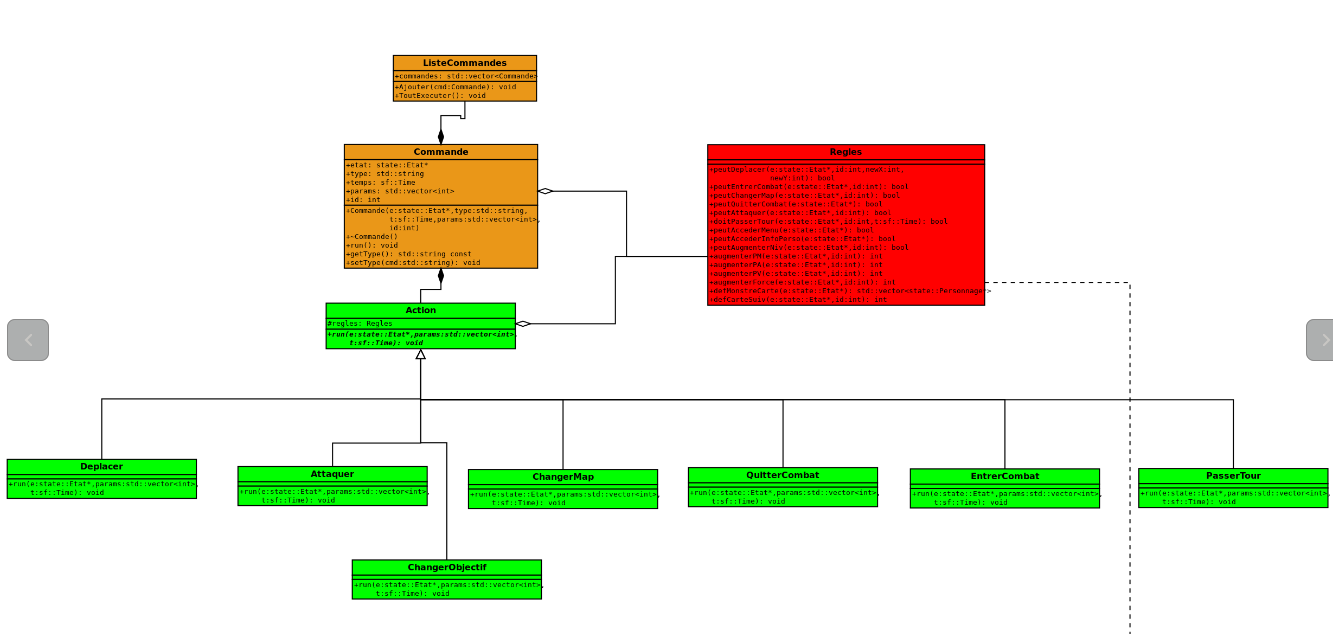
\includegraphics[scale=0.35]{img/engine.png}
  \caption{\emph{Package engine}}
\end{figure}

\newpage

\section{Intelligence Artificielle}
\subsection{Stratégie}
La stratégie d'intelligence artificielle optée dans un premier est basée sur une intelligence simple.
\subsubsection{Intelligence artificielle minimale}
Dans une première approche, une intelligence artificielle minimale est adoptée et est basée selon les déplacements d'un personnages. Les déplacements de l'IA s'effectuent de manière aléatoire selon les quatres directions (nord, sud, est et ouest).
\subsubsection{Intelligence artificielle en combat}
Dans une seconde approche, une intelligence artificielle en combat est implantée et est basée sur une stratégie d'évolution en combat. Cette stratégie consiste à effectuer des déplacements et des attaques précis selon l'ensemble d'heuristiques défini ci-après:
\begin{enumerate}
 
 \item Chercher la cible
  \begin{enumerate}
   \item L'IA choisi la cible ennemi ayant le moins de point de vie (PV).
   \item Si plusieurs ennemis ont le même nombre de PV minimal alors l'IA choisi celui qui est le plus proche.
  \end{enumerate}
 
 \item Se déplacer
  \begin{enumerate}
   \item L'IA se déplace vers sa cible en utilisant autant de point de mouvement (PM) que nécessaire.
  \end{enumerate}
 
 \item Attaquer
  \begin{enumerate}
   \item L'IA attaque sa cible en utilisant autant de point d'action (PA) que nécessaire.
   \item Si la cible et l'IA sont côte à côte alors l'IA effectue une attaque corps à corps.
   \item Sinon, l'IA effectue une attaque à distance.
  \end{enumerate}

\end{enumerate}

\subsubsection{Intelligence artificielle basée sur les arbres de recherche}
Dans une dernière approche, une intelligence artificielle en combat est implantée et est basée sur les arbres de recherche.
Cette stratégie d'intelligence artificielle est fondée suivant l'algorithme du 'MinMax' qui consiste, de manière générale, à maximiser son gain et à minimiser le gain de l'adversaire.
Ainsi, cette stratégie permet au joueur de faire un choix parmi l'ensemble de ses actions possibles en anticipant les choix des actions de son adversaire.


\subsection{Conception logiciel}
\textbf{Classe IA.} Cette classe abstraite permet de créer un objet de type IA qui gère l'exécution des commandes de jeu.

\textbf{Classe IAminimale.} Cette classe hérite de la classe IA et permet de générer des commandes simples de déplacement du personnage.\\

\textbf{Classe IAcombat.} Cette classe hérite de la classe IA et permet de générer des commandes de déplacement et d'attaque précises.

\textbf{Classe IAheuristic.} Cette classe permet de gérer l'ensemble d'heuristiques de l'IA en combat.

\textbf{Classe MinMaxIA.} Cette classe hérite de la classe IA et permet de gérer la stratégie basée sur l'algorithme du MinMax.

\textbf{Classe Arbre.} Cette classe permet de créer un objet de type Arbre.

\textbf{Classe Noeud.} Cette classe permet de créer un objet de type Noeud. Un ensemble de noeuds constitue un arbre.\\

Le tableau ci-dessous résume l'ensemble des classes utiles et présentes pour définir l'intelligence artificielle ainsi que leur rôle respectif.\\

\begin{tabularx}{\textwidth}{ |l|X| }
\hline
   \textbf{Nom} & \textbf{Role}
 \\
\hline

   IA & Cette classe abstraite permet de créer un objet de type IA.
   
Attribut(s): etat
\newline
Méthode(s): IA(), ~IA(), exec\_cmd()
 \\
\hline

    IAminimale & Cette classe hérite de la classe IA permet de généner de simple commandes de déplacement.

Méthode(s): IAminimale(), ~IAminimale(), exec\_cmd()
  \\
\hline

    IAcombat & Cette classe hérité de la classe IA permet de générer des commandes de déplacemement et d'attaque précises.
    
Attribut(s): strat
\newline
Méthode(s): IAcombat(), ~IAcombat(), getHeuristic(), exec\_cmd()
  \\
\hline

    IAheuristic & Cette classe permet de gérer l'ensemble d'heuristiques en combat.

Méthode(s): cible(), posCible(), attaqueCible()
  \\
\hline

    MinMaxIA & Cette classe héritée de la classe IA permet de gérer la stratégie suivant l'algorithme du MinMax.

Attibut(s): tmp\_arbre
\newline
Méthode(s): MinMaxIA(), exec\_cmd()
  \\
\hline

    Arbre & Cette classe permet de créer un objet de type Arbre.
    
Attribut(s): profondeur, racine
\newline
Méthode(s): Arbre(), ~Arbre(), creerArbre(), MinMax()
  \\
\hline

    Noeud & Cette classe permet de créer un objet de type Noeud.
    
Attibut(s): lien, pere, f, id, fils
\newline
Méthode(s): Noeud(), ~Noeud(), createFils(), setF(), getF(), getID(), getLien(), getPere(), MinMax()
  \\
\hline

\end{tabularx}\\ \\*

\begin{figure}[H]
  \centering
  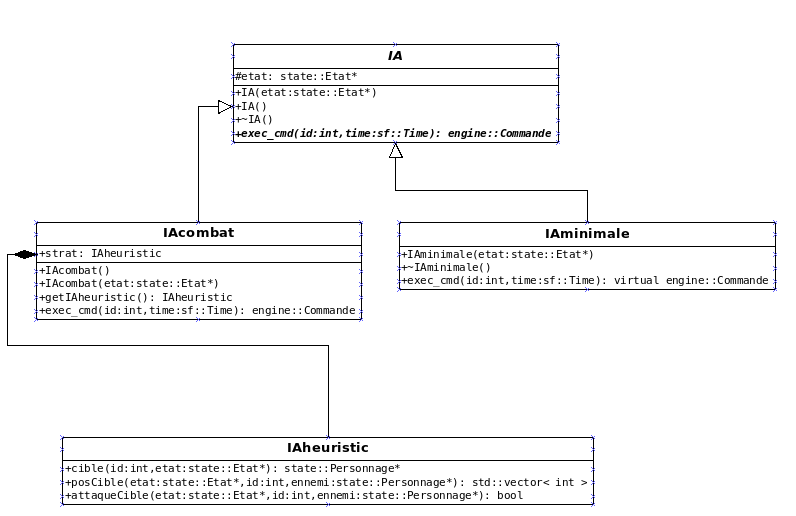
\includegraphics[scale=0.45]{img/ia.png}
  \caption{\emph{Package ia}}
\end{figure}

\section{Modularisation}
  \subsection{Répartition sur différents threads}
  Dans cette partie l'objectif est de distinguer le moteur de jeu de celui du rendu. Pour ce faire, il suffit de placer le moteur du rendu dans un thread et celui du jeu (exécution des commandes) dans un second thread.
  Les commandes ainsi que les notifications du rendu transitent d'un module à un autre. Cette communication entre modules est essentiellement basée sur une stratégie utilisant le ``pattern observer''. En effet, chaque changement d'état est notifié au rendu via ce pattern observable/observer.

  \subsection{Conception Logiciel}
  Pour la conception logiciel concernant la modularisation, il a fallu apporter quelques modifications dans les packages suivants: State, Render et Engine.\\
  
  \textbf{Package State. } Le pattern Observable/Observer a été implanté dans le package State. Ainsi, tout objet héritant de la classe Observer est un observeur et tout objet héritant de la classe Observable devient un objet observé. Ce dernier notifie tout changement éventuel à l'observateur dont il est associé.
  La méthode AccesPerso permet maintenant d'accéder à un mutex d'une source de segfault lors des changements de map.
  
  \textbf{Package Render. } La classe cmdRendu a été ajoutée dans le package Render et permet de stocker les informations nécessaires à l'exécution d'une commande.
  La méthode testChgtMap dans la classe RenduGrille est appelée après une notification de changement de grille.
  La méthode testChgtPerso dans la classe RenduPerso est appeleée après une notification de changement de personnages.
  
  \textbf{Package Engine. } La méthode toutExecuter dans la classe ListeCommandes contient une boucle infinie qui est exécutée dans un thread et copie le buffer, puis le vide et exécute les commandes qu'il contenait.\\
  
  Voici les modifications apportées dans les diagrammes de classes:
  
\begin{figure}[H]
  \centering
  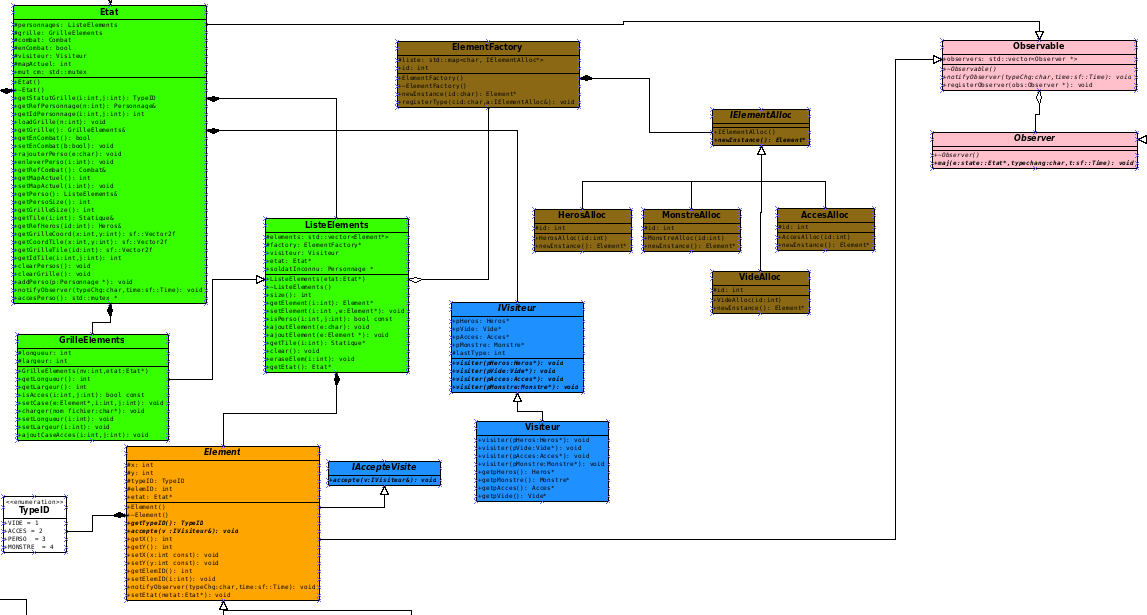
\includegraphics[scale=0.35]{img/state_mod.png}
  \caption{\emph{Modification du Package state}}
\end{figure}
  
\begin{figure}[H]
  \centering
  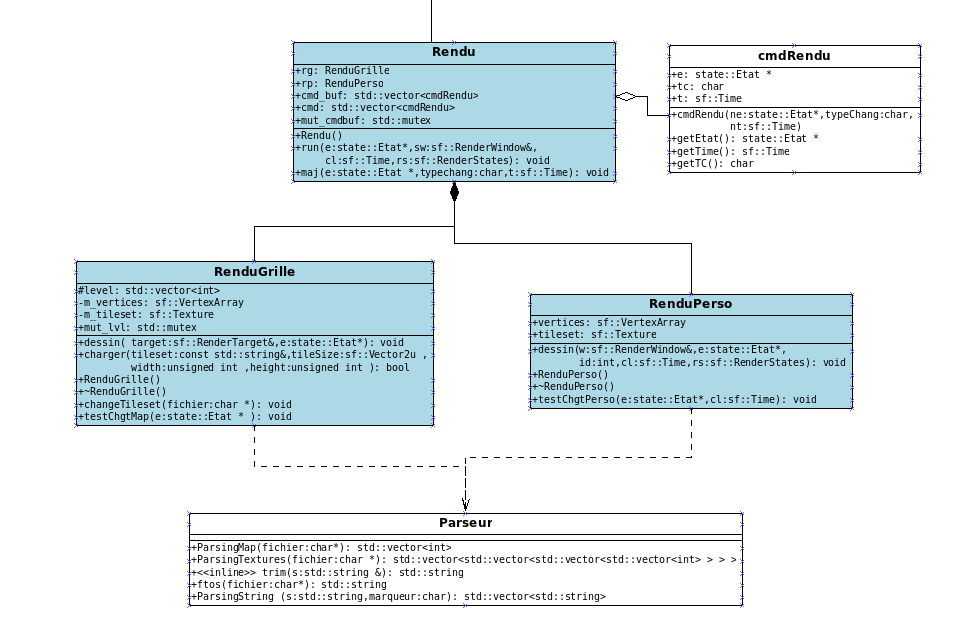
\includegraphics[scale=0.45]{img/rendu_mod.png}
  \caption{\emph{Modification du Package render}}
\end{figure}

\begin{figure}[H]
  \centering
  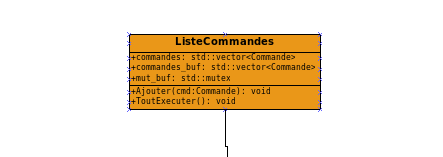
\includegraphics[scale=0.45]{img/engine_mod.png}
  \caption{\emph{Modification du Package engine}}
\end{figure}

\section{Définition des API Web}
Dans cette partie l'objectif est de définir une interface entre le client et le serveur. Pour ce faire, il est nécessaire de définir une API.
Dans ce projet, l'API adoptée est basée sur le format d'API REST et d'un encodage utilisant du JSON.
  \subsection{API basée sur REST/JSON}
  Voici la définition de l'API implantée dans le cadre de ce propjet:\\
  \subsubsection{Services des commandes}
  \textbf{- Méthode PUT } : générer une commande
  
  \begin{enumerate}
   \item \underline{Requête :}
    \begin{enumerate}
     \item Méthode HTTP et URI : PUT/commande/
     \item Données:
	\begin{lstlisting}[language=JSON]
	type: "object",
	properties: {
	  "cmd": { type:string, pattern: "(d|a|cm|im|qc|ec|pt|u)" },
	  "params": { type:array, items: {type: int} },
	  "epoque": { type:int },
	  "perso_id": { type:int},
	},
	required: [ "cmd", "params", "epoque", "perso_id" ]
	\end{lstlisting}      
    \end{enumerate}

   \item \underline{Réponse :}
   \begin{itemize}
    \item Cas où la commande est validée:
    \begin{enumerate}
     \item Status: 200 (= OK)
     \item Données:
	\begin{lstlisting}[language=JSON]
	type: "object",
	properties: {
	  "epoque": { type:int },
	},
	required: [ "epoque" ]
	\end{lstlisting} 
    \end{enumerate}

    \item Cas où la commande n'est pas validée:
    \begin{enumerate}
     \item Status:400 (= BAD\_REQUEST)
     \item Données: Pas de données\\
    \end{enumerate}

    \item Cas où la commande est imcomplète:
    \begin{enumerate}
     \item Status:206 (= PARTIAL\_CONTENT)
     \item Données: Pas de données
    \end{enumerate}
    
   \end{itemize}

  \end{enumerate}

  \newpage
  \textbf{- Méthode GET } : obtenir la commande d'identifiant <epoque>
  
  \begin{enumerate}
   \item \underline{Requête :}
    \begin{enumerate}
     \item Méthode HTTP et URI : GET/commande/<epoque>
     \item Données: Pas de données
	     
    \end{enumerate}

   \item \underline{Réponse :}
   \begin{itemize}
    \item Cas où <epoque> est positif et inférieur à l'époque maximum:
    \begin{enumerate}
     \item Status: 200 (= OK)
     \item Données:
	\begin{lstlisting}[language=JSON]
	type: "object",
	properties: {
	  "cmd": { type:string, pattern: "(d|a|cm|im|qc|ec|pt|u)" },
	  "params": { type:array, items: {type: int} },
	  "epoque": { type:int },
	  "perso_id": { type:int},
	},
	required: [ "cmd", "params", "epoque", "perso_id" ]
	\end{lstlisting} 
    \end{enumerate}

    \item Cas où <epoque> n'existe pas:
    \begin{enumerate}
     \item Status:404 (= NOT\_FOUND)
     \item Données: Pas de données
    \end{enumerate}
    
   \end{itemize}

  \end{enumerate}
  
  \subsubsection{Services des utilisateurs}
  \textbf{- Méthode PUT} : générer une connexion d'un utilisateur
  
  \begin{enumerate}
   \item \underline{Requête :}
    \begin{enumerate}
     \item Méthode HTTP et URI : PUT/connexion/
     \item Données:
	\begin{lstlisting}[language=JSON]
	type: "object",
	properties: {
	  "male": { type:bool },
	},
	required: [ "male" ]
	\end{lstlisting}
	     
    \end{enumerate}

   \item \underline{Réponse :}
   \begin{itemize}
    \item Cas où la connexion est validée:
    \begin{enumerate}
     \item Status: 200 (= OK)
     \item Données:
	\begin{lstlisting}[language=JSON]
	type: "object",
	properties: {
	  "id_perso": { type:int },
	},
	required: [ "id_perso" ]
	\end{lstlisting} 
    \end{enumerate}

    \item Cas où la connexion n'est pas validée:
    \begin{enumerate}
     \item Status:403 (= FORBIDDEN)
     \item Données: Pas de données\\
    \end{enumerate}
    
   \end{itemize}

  \end{enumerate}
  
  \textbf{Méthode DELETE} : gérer la déconnexion de l'utilisateur d'identifiant <id\_perso>
  
  \begin{enumerate}
   \item \underline{Requête :}
    \begin{enumerate}
     \item Méthode HTTP et URI : DELETE/connexion/<id\_perso>
     \item Données:Pas de donnée autre que id\_perso
		     
    \end{enumerate}

   \item \underline{Réponse :}
   \begin{itemize}
    \item Cas où la déconnexion est validée:
    \begin{enumerate}
     \item Status: 200 (= OK)
     \item Données:Pas de données\\	 
    \end{enumerate}
    \item Cas où <id> n'existe pas:
    \begin{enumerate}
     \item Status:404 (= NOT\_FOUND)
     \item Données: Pas de données\\
    \end{enumerate}    
    \item Cas où la déconnexion n'est pas validée:
    \begin{enumerate}
     \item Status:403 (= FORBIDDEN)
     \item Données: Pas de données\\
    \end{enumerate}
    
   \end{itemize}

  \end{enumerate}
  

  \subsection{Conception logiciel}
  Pour implanter cette API, il a fallu définir deux nouveaux packages: le package Server et le package Client.
  
  \textbf{Classe Server.} Cette classe permet de créer un objet de type Server.
  
  \textbf{Classe ServiceException.} Cette classe permet de gérer les exceptions HTTP.
  
  \textbf{Classe AbstractService.} Cette classe abstraite permet de définir les différentes méthodes de l'API REST.
  
  \textbf{CLasse CommandeService.} Cette classe permet de définir les méthodes de l'API REST pour les commandes.
  
  \textbf{Classe UtilisateurService.} Cette classe permet de définir les méthodes de l'API REST pour les utilisateurs.
  
  \textbf{Classe ServiceManager.} Cette classe permet de gérer les différentes requêtes.\\
  
  \textbf{Classe RenduCombat.} Cette classe permet de gérer l'affichage du rendu en mode combat.
  
  \textbf{Classe RectTexte.} Cette classe permet de définir les icônes de type rectangulaire.
  
  \textbf{Classe CerTexte.} Cette classe permet de définir les icônes de type circulaire.
  
  \textbf{OperateurReseau.} Cette classe permet de gérer les opérations en réseau.\\

  
  Le tableau ci-dessous résume l'ensemble des classes utiles et présentes pour définir le package Server ainsi que leur rôle respectif.\\
 
 \begin{tabularx}{\textwidth}{ |l|X| }
\hline
   \textbf{Nom} & \textbf{Role}
 \\
\hline

   Server & Cette classe permet de créer un objet de type Server.
   
Attribut(s): service\_manag
\newline
Méthode(s): Server(),run()
 \\
\hline

    ServiceException & Cette classe permet de gérer les exceptions HTTP.
    
Attribut(s): msg, httpStatus
\newline
Méthode(s): ServiceException(), status(), what()
  \\
\hline

    AbstractService & Cette classe abstraite permet de définir les différentes méthodes de l'API REST.
    
Attribut(s): pattern
\newline
Méthode(s): AbstractService(), ~AbstractService(), getPattern(), setPattern(), get(), post(), put(), remove()
  \\
\hline

    CommandeService & Cette classe permet de définir les méthodes de l'API REST pour les commandes.

Attribut(s): commandes
\newline
Méthode(s): CommandeService(), get(), put()
  \\
\hline

    UtilisateurService & Cette classe permet de définir les méthodes de l'API REST pour les utilisateurs.

Attibut(s): etat
\newline
Méthode(s): UtilisateurService(), put(), remove()
  \\
\hline

    ServiceManager & Cette classe permet de gérer les différentes requêtes.
    
Attribut(s): services
\newline
Méthode(s): registerService(), findService(), queryService()
  \\
\hline

   
\end{tabularx}\\ \\*

\begin{figure}[H]
  \centering
  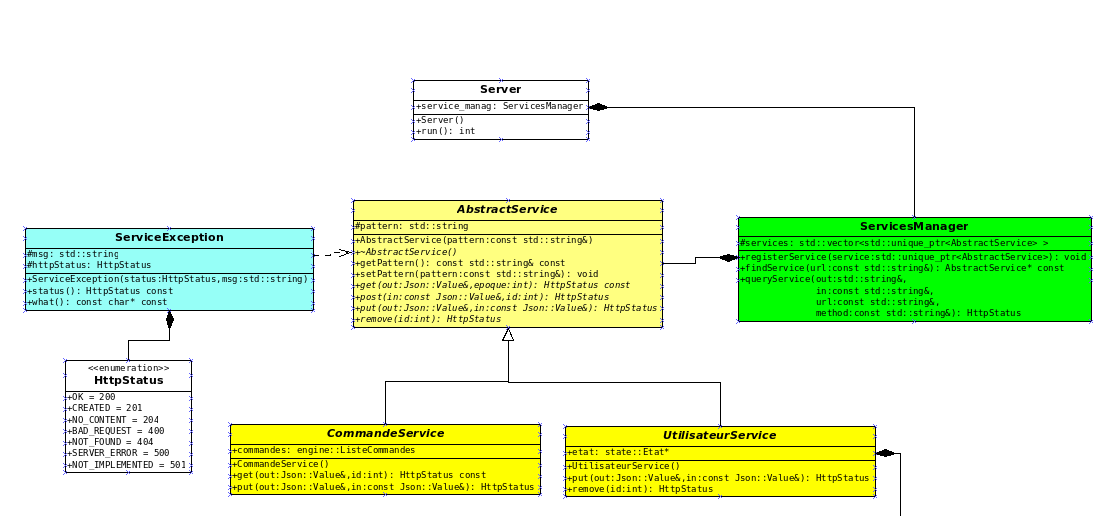
\includegraphics[scale=0.40]{img/package_Server.png}
  \caption{\emph{Package server}}
\end{figure}

Le tableau ci-dessous résume l'ensemble des classes utiles et présentes pour définir le package Client ainsi que leur rôle respectif.\\

\begin{tabularx}{\textwidth}{ |l|X| }
\hline
   \textbf{Nom} & \textbf{Role}
 \\
\hline

   RenduCombat & Cette classe permet de gérer l'affichage du rendu en mode combat.
   
Attribut(s): iconeAttaqueDist, iconeAttaqueCAC, iconePA, iconePM, iconeVie, iconeTemps, iconeTourSuiv
\newline
Méthode(s): dessin(), RenduCombat(),~RenduCombat()
 \\
\hline

    RectTexte & Cette classe permet de définir les icônes de type rectangulaire.
    
Attribut(s): texte, rect, font
\newline
Méthode(s): ChangeText(), RectTexte(), ~RectTexte()
  \\
\hline

    CerTexte & Cette classe permet de définir les icônes de type circulaire.
    
Attribut(s): texte, cercle, font
\newline
Méthode(s): ChangeTexte(), CerTexte(), ~CerTexte()
  \\
\hline

    OperateurReseau & Cette classe permet de gérer les opérations en réseau.

Attribut(s): in\_cmd\_list, out\_cmd\_list, in\_th\_buf, mut\_in, mut\_out, sender, active, epoque\_locale, e, http
\newline
Méthode(s): th\_in(), th\_out(), getCmd(), putCmd(), OperateurReseau(), ~OperateurReseau(), run()
  \\
\hline

      
\end{tabularx}\\ \\*

\begin{figure}[H]
  \centering
  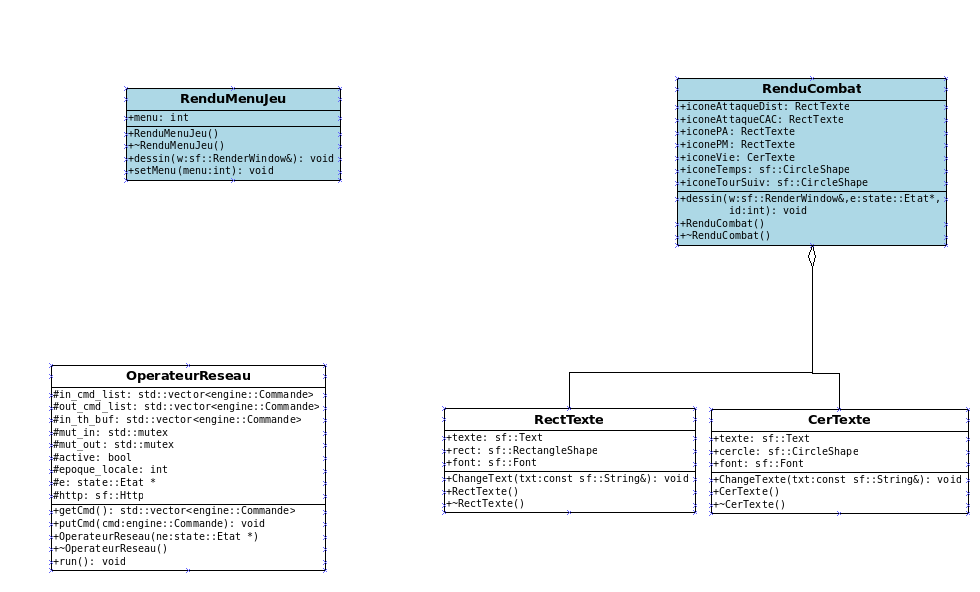
\includegraphics[scale=0.45]{img/package_Client.png}
  \caption{\emph{Package client}}
\end{figure}

\end{document}\grid
